%\documentclass[11pt]{report}
\documentclass[12pt, twoside, ngerman]{report} 
%\documentclass[12pt,twoside]{report}
% \documentclass{article}
\usepackage{amssymb}
\usepackage{algpseudocode}
\usepackage{algorithm}
\usepackage{setspace}
\usepackage{graphicx}
\graphicspath{ {./images/} }
\usepackage{hyperref}
\usepackage{siunitx}
\usepackage{amsmath}
\usepackage{caption}
\usepackage{subcaption}
\usepackage{geometry}
\usepackage[english]{babel}
\usepackage[T1]{fontenc}
\usepackage[utf8]{inputenc}


\usepackage{tikz}
\usetikzlibrary{positioning}
% \usetikzlibrary{graphdrawing.trees}

\usepackage{booktabs}

\hypersetup{
    colorlinks=false,
    linkcolor=blue,
    filecolor=magenta,
    urlcolor=cyan,
}

% Commenting out another way to write the title.
% \title{MSc Thesis - Ranking Loss Surrogates}

\iffalse    
\author{
        Abdus Salam Khazi [
        \href{mailto:abdus.khazi@students.uni-freiburg.de}
                {Email} ]\\ \\
        \href{https://github.com/abduskhazi/ranking-loss-surrogates.git}
                {Github Repository} \cite{github_repository} \\ \\
        Supervisors:
        \begin{tabular}{ll}
             JProf. Josif Grabocka \&
			Sebastian Pineda
		\end{tabular}
       }
\fi


\begin{document}

\newgeometry{
    top=1.5in,
    bottom=1.5in,
    outer=1.75in,
    inner=1.25in,
    }

\title{
{\LARGE Master's Thesis}
\vspace{20pt}
\hrule
\vspace{20pt}
\textbf{Hyperparameter Optimization using Ranking Loss Surrogates}
\vspace{20pt}
\hrule
\vspace{20pt}
\author{{\LARGE Abdus Salam Khazi}}
\date{\LARGE \today}
\begin{figure}[h]
    \centering
    
\includegraphics[width=50mm]{images/Logo.png}
\end{figure}
\large{Albert-Ludwigs-University Freiburg
\\Representation Learning Department}
}
    
\pagenumbering{gobble}

\maketitle
    

% \date{}

\chapter*{Declaration \thispagestyle{empty}}


I hereby declare, that I am the sole author and composer of my thesis and that no other sources or learning aids, other than those listed, have been used. Furthermore, I declare that I have acknowledged the work of others by providing detailed references of said work. 

I hereby also declare, that my Thesis has not been prepared for another examination or assignment, either wholly or excerpts thereof

\vspace{100pt}

\begin{minipage}{2in}
\textbf{\underline{\hspace{100pt}}} \\
Place, Date
\end{minipage}
\hfill
\begin{minipage}{1.3in}
\textbf{\underline{\hspace{100pt}}} \\
Signature
\end{minipage}

\newpage
\pagenumbering{roman}
\begin{abstract}

Abstract goes here

\end{abstract}

\newpage

\tableofcontents
\newpage
\newpage

\pagenumbering{arabic}

\chapter{Introduction}

The performance of any machine learning model is sensitive to the hyper-parameters used during the model training. 
Instead of using a new model type, it is more helpful to tune the hyper-parameters of an existing model to improve its performance.
Learning the best hyper-parameter for an ML model is called, Hyperparameter optimization (HPO in short).

The true evaluation of a hyperparameter optimisation objective function is computationally very expensive. 
Researchers have tried to get around this problem by proposing model based HPO algorithms.
In these methods,  the true objective function is modelled by a cheap surrogate function of high representational capacity.
For example,  the Sequential Model Based Optimization (SMBO)~\cite{NIPS2011_86e8f7ab} algorithm is a very important algorithm that iterates between learning a model given a few HP configuration evaluations and using the model to propose the next candidate to evaluate.

This thesis studies various existing approaches to HPO and proposes a new idea for the same using the concept of ranking.
The proposed idea in this thesis is called \textbf{Hyperparamter Optimization using Ranking Loss Surrogates}. 
The results obtained using this model are compared against the state-of-the-art results obtained using models like FSBO,  RGPE,  TAF, and others. 

\label{ProblemOverviewlabel}
\section{Objective}
The aim is to study ranking loss surrogates in the context of Hyperparameter optimization.

\section{Overview}
This sections contains the overview of the paper and how the thesis report is organised.


\chapter{Related Work}\label{chap:relatedWork}

In this chapter,  the hyper-parameter optimization problem is first defined concretely.
Then, the various approaches already used to do the HP optimization are discussed.
Subsequently,  some important concepts that the thesis uses to build the proposed model are also discussed.

\section{Hyper Parameter Optimization}
To find out the best hyper-parameter for any machine learning model $m$, we must first quantify a given hyper-parameter configuration $\textbf{x}$ by a real-valued number $v \in \mathbb{R}$.
If we define that
$$
\textbf{x}_1 \succ  \textbf{x}_2 \iff v_{\textbf{x}_1} < v_{\textbf{x}_2}
$$
then HPO can be defined mathematically by an abstract function, say,  $f(\textbf{x}) \mapsto \mathbb{R}$ as
$$
     \underset{\rm \textbf{x}}{\rm argmin}  f(\textbf{x}) \;\;\;  \forall \textbf{x} \in \mathbb{S}
$$
where $\mathbb{S}$ is the hyper-parameter search space.

This function $f(\textbf{x}) \mapsto \mathbb{R}$ is evaluated in the following chronological steps:
\begin{enumerate}
\item Using a given hyper-parameter configuration $\textbf{x}$,  we train our model $m$ to obtain the model $m^{trained}_\textbf{x}$. It consists of learning the parameters of our model, E.g. learning the weights and biases of a Deep Neural Network.
We use the training data to learn this model.
\item The validation data is passed through $m^{trained}_\textbf{x}$ to obtain the required results.
These results are evaluated based on an evaluation criterion '$\textrm{eval}$'. This criterion is different for different problems, e.g. Regression, Classification, etc.
The result of this evaluation is a real-value that gives a score for the configuration $\textbf{x}$.
\end{enumerate}

Hence the function $f(\textbf{x}) \mapsto \mathbb{R}$ can be written as 
$$
f(m^{trained}_\textbf{x} (\textrm{Data}_\textrm{val})) \mapsto \mathbb{R}
$$

Finally, the HPO problem can be defined using the following equation:
\begin{equation}\label{eq:hpoobjectivefunc}
\underset{\rm \textbf{x}}{\rm argmin} \;\; f(m^{trained}_\textbf{x} (\textrm{Data}_\textrm{val})) \mapsto \mathbb{R}   \;\;\;  \forall \textbf{x} \in \mathbb{S}
\end{equation}

\subsubsection{HPO Constraints}

Hyperparameter optimization is different from other optimization methods because it has different constraints~\cite{bayesianOptimizationTutorial}.
It is because of the peculiar properties of the hyper-parameter search spaces.
Finding out the correct hyper-parameter setting is generally not feasible using a brute-force approach (trying out all possible combinations of hyper-parameters) because the search space itself has many dimensions, and the search space may be continuous.
More specifically,  some of the important constraints of this optimization problem are:

\begin{enumerate}
\item The evaluation of a given HPO configuration is computationally expensive.
\item It is a non-convex optimization problem.
\item The process of getting $m^{trained}_\textbf{x}$ from $m$ is stochastic hence the value $v_{\textbf{x}}$ is noisy.
\item Some dimensions have conditional constraints. The values of some dimensions may depend on the values of others. For example, the number of neurons in layer 3 only makes sense if we have 3 or more layers in a neural network.
\item The search space is hybrid in terms of continuity. Some of the dimensions (variables) may be continuous, while others may be discrete.
Using a gradient method is hence not trivial.
\end{enumerate}

To deal with the constraints of HPO problems, researchers have used different strategies for developing HPO algorithms and models.
Some of the more prominent approaches are Black-Box HPO, 
Multi-fidelity HPO and Online HPO.

\subsection{Black-box HPO}
In this approach the HPO objective function $f$ in equation~\ref{eq:hpoobjectivefunc}
is treated as a blackbox.
The problem is thus generalised to finding a global optima of $f$.
Some of the straightforward black-box HPO methods include Manual Search,  Grid Search and Random Search.
The optimization technique called Bayesian optimization gives us a more sophisticated mechanism to deal with this problem. 

Manual Search in the HPO search space is feasible when we have expert knowledge of the problem and the given model. 
The idea is to select configurations step by step by observing the results obtained
so that we do not waste computation time evaluating similar configurations through intuition.
This approach may be helpful for small models with lesser constraints.
However, as the HPO search space becomes very large or conditional constraints become too complex, the selection of configurations becomes more and more difficult.
Hence a more systematic and automated approach is more practical.

Grid search is a more systematic approach in which we divide the search space into grid points similar to ones in a Euclidean graph.
Let there be $m$ dimensions in the search space $\mathbb{S}$. Let the selected number of values for each dimension be $n_1, n_2, ... n_m$. In the case of a discrete variable, the selected values will be a subset of the possible values, whereas, in the case of a continuous variable, we need to select the values based on a selected granularity.
The cross-product of the selected subsets gives us the configurations to be evaluated. Hence, the number of configurations to evaluate will be $n_1 * n_2 * ... n_m$.
The number of configurations we need to evaluate in this approach becomes a big issue for this method as the dimensions of the search spaces increase.
Hence this approach becomes intractability for large search spaces.

\begin{figure}[htb]
  \centering
    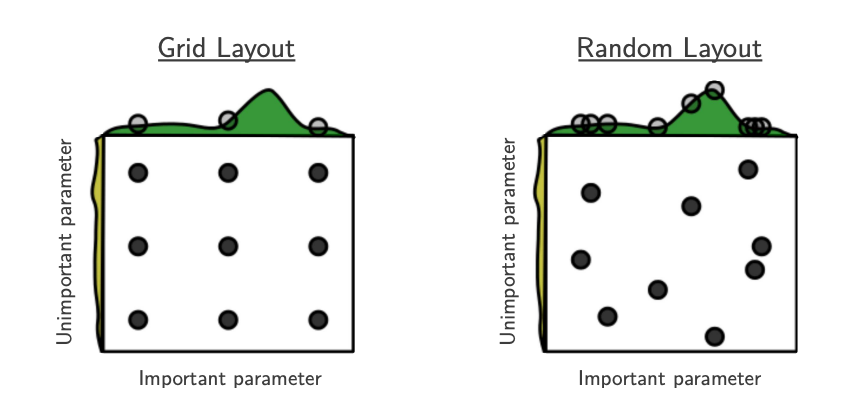
\includegraphics[scale=0.8]{images/rsgsexample}
    \caption{Illustrates Grid search and Random search in the case where 2 parameters are not equally important.  Adpated from~\cite{rshpoarticle}.}
    \label{fig:rshpofig}
\end{figure}

One issue with the Grid Search approach is that we assume that all dimensions in the HPO search space are equally important. It is not the case in many HPO problems.  The Grid layout in Figure~\ref{fig:rshpofig}(left) shows illustrates this.  For example, the learning rate in deep neural networks is much more important than many other parameters. If dimension $p$ is the most important in the search space, then it makes sense to evaluate more values of $p$. Random Search helps us solve this problem. 
The Random layout in Figure~\ref{fig:rshpofig}(right) illustrates this. 
Hence Random Search can be used as a trivial baseline for comparing other HPO models.

One advantage of these methods is that there are no restrictions on the HPO search spaces. Hence, they are suitable for any HPO problem at hand.
On the other hand, these methods are non-probabilistic.
Hence they cannot deal with noisy evaluations of the HPO configuration well.
Moreover, these methods are computationally expensive. The reason is that they do not use surrogate evaluators and hence train and evaluate the whole model.
Also, these search methods give us optimal HPO configurations only by chance.
\subsubsection{Bayesian Optimization}

Bayesian optimization tries to solve both computational costs and noisy evaluations of our objective function $f$.
It does this by building a model of the HPO objective function. This model is called a surrogate function.
Bayesian optimization uses known evaluations as its data to build the surrogate model. The data is of the form \{x, f(x)\} pairs.
The surrogate model is a probabilistic model. Hence, it also learns about the noise in the evaluations of the objective function.

The core procedure of the optimization process is the following:
\begin{itemize}
\item From known data $D = {(x_1, f(x_1)), (x_2, f(x_2)), (x_3, f(x_3)) .... }$, build a probabilistic model that learns the mean and variance of the objective function
\item Use the surrogate to sample the next best HPO configuration x' using a function known as acquisition function. Evaluate f(x').
\item Append (x', f(x')) to D and repeat the process.
\end{itemize}

The above process repeats till the computational resources are finished (here time) or we find an acceptable HPO configuration.
This procedure is also called SMBO (Sequential model-based Optimization).
The procedure alternates between collecting data and fitting the model with the 
collected data~\cite{SMBOPaper}.

Hence, there are two essential components of Bayesian optimization:

\begin{itemize}
\item Probabilistic surrogate model of the objective function.  Some surrogates are discussed in detail in the subsequent sections in this chapter.
\item The acquisition function
\end{itemize}

\subsubsection{Acquisition functions}
The acquisition functions used in the bayesian optimization need to do balance exploitation of information from the known/observed data points and exploration of unknown data points in the domain.
The following functions are some of the most prominent acquisition functions found in the literature~\cite{GPTutorial}
\begin{itemize}
\item \textbf{Upper Confidence Bound (UCB)}: It returns the best possible hyperparameter configuration using a linear combination of the mean and the standard deviation.
\item \textbf{Probability of Improvement}: It gives the probability with which we can get a better hyperparameter configuration than the incumbent best configuration.
\item \textbf{Expected Improvement}: Given a Gaussian distribution at a new input point, it finds the expectation of improvement i.e ($f(x) - f_{max}$) over the part of normal that is greater than $f_{max}$.
\end{itemize}

 \textbf{Expected Improvement} acquisition function is used all around the thesis in order to do a fair comparison of the models and algorithms.

\subsection{Online HPO}
Traditionally to evaluate and select a new HP configuration,  the objective function $f$ is fully evaluated.
In the most general sense this can be applied to both discrete and continuous HP search spaces.
Some advanced methods have proposed even gradient based HP optimization.

For example,  Maclaurin et al.~\cite{hypergradient} proposed a relatively cheap method to obtain hyper gradients i.e gradients of hyper parameters with respect to the whole objective function $f$.
Further,  Franceschi et al.~\cite{HPOAsBilevelOptimization} formulated the whole HPO problem as a bi level optimization problem~\cite{hutterneuripstutorial}.

In all these methods as the hyper parameters and the parameters of the model are being learnt disjointly,  they can be referred to as offline HPO.
The idea of online HPO is that it tries to evaluate and update the HP configuration during the training of the model itself.

Sometimes only a single hyper parameter is learnt online.
For example,  Baydin et al.~\cite{onlineLearningRateUpdate},  proposes the online learning of the learning rate.  They target this hyper parameter because it is the single most important hyper parameter.
In other times all parameters may be learnt.
For example,  Luketina el at. ~\cite{gradientbasedHPOtuning} proposes to interleave the updating of training parameters and hyper parameters.


\subsection{Multi-fidelity HPO}
If we treat our HPO objective function $f$ as a black box function,  we would need to evaluate equation~\ref{eq:hpoobjectivefunc} fully.
This is prohibitively expensive as evaluating a single HP configuration may take days~\cite{hutter2019automated}.
Multi-fidelity hyper parameter optimization tries to solve this problem by evaluating the HP candidates on cheap functions $f_{approx}$ that approximate the objective function $f$.

Here, $f_{approx}$  is called a fidelity as it copies or reproduces the true objective function upto some degree.
For example,  a fidelity could be evaluation of the HP configuration on only a subset of data,  the evaluation of the HP on downscaled image data or learning only for a few epochs etc.
The idea is to trade off between the performance of the approximate function and its optimization accuracy such that we get best selection of HP using the least compute power.
Since the true evaluation of HP configuration using $f$ is not done,  it is an approximate optimization technique.

The technique does not belong to the black box HPO domain.
This can be understood very clearly if we take the example of the "few epochs" fidelity.
Clearly,  the optimization algorithm looks into the training process the learns the objective function to prematurely exit it if need be.
Thus getting a feedback from within the "black box" of the HPO objective function.

The reason this technique is called multi-fidelity is because it may use different fidelities within the optimization process to get the best HP configuration.
For example,  while using successive having technique~\cite{successivehalving} for HPO one can start with a given "budget fidelity" for example - defined number of epochs or defined amount of training time.
At each step of the optimization process,  the budget is doubled and the worst performing HP configurations are eliminated for the next step.
Hence it uses "multiple" fidelities during the optimization process.


\section{Transfer-learning for HPO}

The HPO methods discussed so far,  evaluate each HP configuration from scratch.
In addition to being computationally inefficient,  it is contrary to how humans learn.
Humans use prior experience that they have accumulated and condition their actions on this knowledge.
Any machine learning mechanism that uses this concept is called a transfer learning method~\cite{Weiss2016}.

This concept of transfer learning can be utilized to accelerate HPO.
For example,  Gomes et al. ~\cite{svmhpmetalearnt} propose to meta learn a set of good HP configurations for the SVM.
They propose that if we learn HP configurations that worked well previously,  then there is high chance of finding that a new SVM model also works with these parameters well.
This concept of warm starting the HP optimization is also proposed by Reif et al.~\cite{metalearningwarmstartpaper} albeit for genetic algorithms.

There are 2 broad ways to transfer knowledge for doing HP optimization - By learning surrogates or by doing warm starting of initial configurations.

\subsection{Warm starting}

Before running any HPO method,  normally experts study the data being used to train the given model.
Based on their study they suggest a few initial HP configurations that have worked well for similar datasets according to their experience.
These initial configurations are evaluated for the given model and the evaluated values act as a starting point (or hinge) for the HPO method.
This is essentially automated by the warm starting method~\cite{Feurer2014UsingMT}.

In the above mentioned papers ~\cite{svmhpmetalearnt},  ~\cite{metalearningwarmstartpaper} the authors use the meta learnt HP configurations as starting points for finding the optima in the HP response surface.
Additionally this idea was also proposed for the SMBO optimization algorithm by Feurer et al. ~\cite{Feurer2014UsingMT}.


\subsection{Meta-learning of surrogates}

HPO models that use surrogates like SMBO,  have an additional gateway through which previous knowledge can be injected.
The idea is to meta-learn the surrogate using previously stored meta-data from similar tasks.
This is used by Schilling et al.~\cite{Schilling2016ScalableHO} in which they learn a collection of Gaussian models for each previously similar dataset due to computational constraints.
They then use the collection of GPs as a surrogate for the SMBO procedure.
Another flavour of this approach was proposed  by Feurer et al.~\cite{Feurer2018ScalableMF} proposed the use of rank weighted GP Ensembles (RGPE) surrogates meta-learnt from previous meta data.

This meta learnt surrogate can be used in 2 different ways during the HPO optimization procedure.
For example in SMBO,  one could use it without any modification (aka fine tuning) to suggest the next best candidate to evaluate from a given HP configuration list.
On the other hand the surrogate can be further meta trained (aka fine tuned) using the available target task meta data. 

Using meta learning of surrogates,  this thesis proposes a new surrogate model.

\section{Types of Surrogates for BO in HPO}
Hyperparameter optimization using Sequential Model Based Optimization (SMBO)~\cite{NIPS2011_86e8f7ab} is a convenient method proposed in the literature.
However,  the performance of this method is heavily reliant on how well the surrogate (model in S\textbf{M}BO) models the true HPO objective.
In this section,  we discuss in details some of the powerful surrogates that may be used with SMBO.

\subsection{Gaussian Processes}

Gaussian processes~\cite{GPTutorial} are predictive machine learning models that work well with few data points (or data pairs). 
They are inherently capable of modeling uncertainty.
Hence, they are used widely in problems such as hyperparameter optimization, where uncertainty estimation is essential.
In this section, we briefly explain the Gaussian process regression intuitively.

Before we proceed,  we need to understand normal (Gaussian) distributions. 
Consider a scalar random variable $X$ that is distributed normally  (a.k.a Gaussian distribution) around a mean $\mu$ with a variance of $\sigma^2$.
The following equation defines the probability density function (PDF) of $X$: 
$$
P_X(x) = \frac{1}{\sqrt[2]{2\pi}\sigma}\exp\left(- \frac{(x - \mu)^2}{2\sigma^2}\right)
$$
Here, $X$ represents the random variable, and $x$ represents an instance of the variable~\cite{GPTutorial}.
In this case,  the mean $\mu$,  variance $\sigma^2$, and any sample $x$ are all scalars.

If the random variable $\textbf{X}$ is a vector in $\mathbb{R}^d$ where $d \in I^{+}$,  then each component of the vector can be considered as a random variable.
In this case the mean $\boldsymbol{\mu} \in \mathbb{R}^d$ whereas variance, represented by $\Sigma$, is in the $R^{d \times d}$ space.
It is because the variance of all components in any valued vector random variable $\textbf{X}$ should contain the following two types of variance
\begin{itemize}
\item Variance of a vector component w.r.t itself.
$d$ diagonal values of the matrix $\Sigma$ represent this variance.
\item Variance of each vector component w.r.t all other components. These variances are represented by the upper/lower triangular values in the matrix $\Sigma$.
\end{itemize}
The matrix $\Sigma$, also known as the Covariance matrix, thus has all values necessary to represent the variance of any vector-valued random variable.


The probability density function of a vector valued variable $\textbf{X} \in \mathbb{R}^d$ with a mean $\boldsymbol{\mu}$ and covariance matrix $\Sigma$ is given by~\cite{MITMLBook}:

$$
\mathcal{N}(\textbf{x} | \boldsymbol{\mu},  \Sigma) = 
\frac{1}{(2\pi)^{\frac{d}{2}} |\Sigma|^{\frac{d}{2}}}
\exp\left( - \frac{1}{2} (\textbf{x} - \boldsymbol{\mu})^T  \Sigma^{-1}   (\textbf{x} - \boldsymbol{\mu}) \right)
$$
This equation defines the PDF of a multivariate normal distribution.

The core idea used in the Gaussian processes is that functions can be considered as vectors of infinite dimensions.
Consider any function $f$ that has a domain $\mathbb{R}$.
If $f$ is considered to be a vector in $\mathbb{R}^{\infty}$,
then each point $i \in \mathbb{R}$  can be represented by a component $f_i$ of the function $f$.
A function,  hence,  is nothing but a sample from $\mathbb{R}^{\infty}$.
Unfortunately, functions sampled from $\mathbb{R}^{\infty}$ are too general and not useful by themselves.

The idea of Gaussian processes is to sample smooth functions from $\mathbb{R}^{\infty}$.
In any smooth function $f$, if any point $g$ is close to $x$ in the domain of $f$, then $f(g) \approx f(x)$.
It is mathematically represented by the following equation:
$$
\lim_{\delta x \to 0} f_{x + \delta x} \approx f^{+}_x  \;\; \textrm{and} \;\; 
\lim_{\delta x \to 0} f_{x - \delta x} \approx f^{-}_x 
$$
$$\;\; \textrm{where} \;\; \delta x > 0 \;\; \textrm{and} \;\; x, \delta x \in \mathbb{R}
$$
The above definition is nothing but the definition of a smooth function in terms of vector notation. 
Moreover, nearby components of $f$ "vary" similarly w.r.t each other.
These properties can be naturally encoded using a covariance matrix.
Hence, we obtain smooth functions if we sample them from a multivariate normal distribution with the required covariance matrix.
The Gaussian process restricts the function sample space to a multivariate normal distribution.

The similarity between 2 points in a domain is defined by a function called \textbf{kernel} in Gaussian processes.
Using this kernel function, the values in the required covariance matrix are populated.
The smoothness of the sampled function $f$ is controlled by the kernel in the GP process.
Formally kernel $k$ is defined as,
$$
k(\textbf{x}, \textbf{x'}) \mapsto \mathbb{R}
$$

Here, $\textbf{x}, \textbf{x'}$ belong to a domain in the most abstract sense.
For example,  when the input domain is a euclidean space,  $\textbf{x} \in \mathbb{R}^{\mathbb{I}^+}$.

Some well known kernels are:
\begin{itemize}
\item \textbf{Radial Basis Function Kernel}
\item \textbf{Matern Kernel}
\item \textbf{Periodic Kernel}
\end{itemize}

Finally,  a Gaussian Process specifies that any new observation $y^*$ for input $\textbf{x}^*$,  is jointly normally distributed with known observations $\textbf{y}$ (corresponding to the input $\textbf{X}$) such that
\begin{align}
    Pr\left( \begin{bmatrix}
           \textbf{y} \\
           y^*
         \end{bmatrix}
         \right)
         &=  \mathcal{N}\left(m(\textbf{X}), \mathbf{\Sigma}\right)
\end{align}

Here, $m(\textbf{X})$ is the mean of the vectors which is commonly taken as $\textbf{0}$.
$\mathbf{\Sigma}$ is the covariance matrix defined as
$$
\mathbf{\Sigma} = \begin{bmatrix}
           \textbf{K} & \textbf{K}_* \\
           \textbf{K}_*^T & \textbf{K}_{**}
         \end{bmatrix}
$$
  Where $\textbf{K} = k(\textbf{X}, \textbf{X})$,  $\textbf{K}_*  =  k(\textbf{X}, \textbf{x}_*)$ and $\textbf{K}_{**} = k(\textbf{x}_*,  \textbf{x}_*)$ for any given kernel $k$~\cite{GPTutorial}.
  Due to the robustness of the GP process, we use this as one of the baselines in our thesis.

\subsection{Random Regression Forest}
     The core idea of this model is to train a Random Regression Forest, using the known data as in any SMBO procedure~\cite{SMBOPaper}.
Random regression forests are an ensemble of regression trees. 
This property is used to our advantage to predict the mean and the variance. 
The mean of the prediction of all the trees is the mean of the surrogate model.
The variance in the prediction of all trees is the variance of the surrogate model.

   The advantages of this model are
   \begin{itemize}
   \item It can handle both continuous and discrete variables trivially without any modifications to the model.
The data splitting during training is done using any variable be it discrete or continuous.
	\item It can handle conditional variables, unlike Gaussian processes, by making sure that data is not split based on a variable till it is guaranteed that no conditionality is broken by the split.
   \end{itemize}

\subsection{Bayesian Neural Networks}
\subsection{Neural Networks}
they don't work great, because they cant model uncertainty). Uncertainty can be modeled directly, or through ensembles.

\section{Types of Losses}
\subsection{BO with GP uses negative log likelihood}
It is not clear whether pointwise losses (regression as in GP) are the correct way to model HPO responses, because we only care for the minima regions (best performing configurations), and not for estimating all observations accurately.

\subsection{Ranking loss could be the answer in modeling hp optima better}
\subsubsection{Pointwise}
\subsubsection{Pairwise}
\subsubsection{Listwise}

\section{Set-modeling with Neural Networks}
In HPO we make predictions based on a set of observations, therefore, in this thesis, I explore the benefit of contextualizing surrogate models on the observations so far.
\subsection{Set-transformers}
\subsection{Deep Sets}



In the remainder of this section, we discuss some sophisticated probabilistic models for doing HPO that use surrogates to reduce computational costs.



There are many probabilistic models such as Random Forests, Gaussian Processes, Tree parson Estimators, etc.
But for the purpose of this thesis, we briefly mention Random forests and discuss in-depth the Gaussian processes.


\iffalse
% Research Paper: https://arxiv.org/pdf/1612.01474.pdf
  2 
  3 Problem: How can we use DNN to quantify uncertainty in a prediction?
  4 
  5 Solutions Previously:
  6     1. Bayesian neural networks.
  7        A prior over weights and biases is specified. Given the data, a posterior is calculated.
  8        Hard and complex to train.
  9 
 10     2. Ensemble approach. E.g Using Monte Carlo Dropout during evaluation. (Behaves like an ensemble)
 11        Consider 10 predictions in an ensemble. Using these, we could calculate the variance and the
 12        mean of the gaussian. Example: Section 3.2 Regression on toy datasets.
 13 
 14 Evaluation of Predictive uncertainties:
 15     Scoring rules - Measure quality of predictive uncertainty.
 16     Out of distribution uncertainty
 17 
 18 Contributions by authors:
 19     Non Bayesian approach.
 20     Ensemble of neural networks.
 21     Adversarial training for smooth predictions (Adversarial training is optional as it improves the prediction uncertainty quality only     in some cases).
 22 
 23 
 24 Proposed Implementation:
% 25     Given theta are NN parameters, we need to predict p_theta(y|x).
 26     p = distribution over real values in regression
 27     p = Discrete probablistic distribution for classification.
 28 
 29     3 step approach - Proper scoring rules, adversarial training and ensemble of NNs.
 30 
 31 Understanding proper scoring rules:
 32     A scoring function gives a numerical value to the predictive distribution.
 33     The better the predictive distribution calibrated to the actual distribution the better the score.
 34     Compare p (prediction distribution) and q (original distribution). The closer p and q are the better the score.
 
 Observations:
 37    How to combine regression and classification problems in deep ensembles - This is possible by having the correct loss function. For ex    ample addition of different parameters.
 38    Understand the intuition behind the adversarial examples y = nn(x). We assume that nn is a smooth function hence the small
 39    change in x should only have a small change in y. Hence nn( neighbourhood(x) ) = y
% 40    For good training use 2^N examples for neighbourhood.
 41    Used a custom NN architecture rather than using 1 hidden layer with 50/100 units depending on the data available.
 42    This is because the architecture given in the paper was not helpful.
 43 
 44 Evaluations of confidence vs accuracy.
 45     The deep ensembles seem to have a better accuracy with higher confidence as compared to MC-Dropout.
 46 
 47 For Using Deep Ensembles for HPO:
 48     We can only use the regression version of the research because the objective scoring is a real valued number
 49     How to model discrete input dimensions as inputs into the Deep Ensemble?
 50 
 51 Doubts:
 52     Could not understand section 3.5 last paragraph correctly.
 53 
\fi

\iffalse
\section{RGPE}
Read the FSBO paper and write the summary like that or read  the RGPE paper
This section is necessary because our model performs similar to this

\section{TAG}
Read the TAG paper.
Some other model if also necessary and you mention this in your report.
\fi

% \section{Deep Kernel Learning}

\iffalse
Paper: https://arxiv.org/pdf/2101.07667.pdf

Problem Domain: Hyperparameter searching.
Keyword: Use Deep Kernel surrogates

Key points:
    1. Use transfer learning surrogates to get faster convergence
    2. Treat HPO as a few shot learning problem (In the context of transfer learning)
    3. Use kernel k(phi(x), phi(x')) where phi is a neural network that transforms x to a latent vector
    4. Learn parameters of phi(W) and kernel(theta) together based on historical meta data
    5. Fine tune both W and theta based on the given task. If possible use warm start for initialization.
    6. Learn output range variance by creating augumented tasks.

Conceptual points:
    1. The deep kernel learnt does not have any task dependent parameters.
       The task dependent parameters are marginalized out.
       Hence finetuning during test time (after pretraining) should be complete.

Quick note on expected improvement.
    First the mean and variance is calculated for the target Hyperparameter Setting.
    Considering the mean and variance of a particular HP, we calculate the following:
%        Remove y_max from the set of all values of f(x) and lowerbound it by 0.
 %       Multiply the above value with the probability of the gaussian curve N(predicted_mean, predicted_variance)
        For a continous curve we need to integrate.
    Then we get the Expected Improvement for this HP setting.


Gaussian Processes:
    The output is considered to be a random variable.
    When have more than 1 data point, the output becomes a multivariate normal
        The output is a joint gaussian distribution.

Personal points (Probability vs Likelihood)
    Probability and likelihood are reverse in nature.
    Probability starts with a given set of parameters and caculates the probability of a given outcome to occur
    Likelihood starts with a given outcome, and we would like to determine the parameters.

    Marginal likelihood (Likelihood after marginalization of some parameters)
        integrates the effects of parameters that are not of your interest.

Note:
    Warm start is not essential for us. (It is not the main contribution of the paper)

Main motive of deep kernel learning:
    Learn the kernel function in the gaussian process.

How to do implementation with FSBO with HPO-B Metadataset?
There are 16 search spaces (model optmizations here)
    The train test split is already done metatraindata has the training data and metatest data has the test data.
    What about validation?? Really required?
    The search space id can be used for identifying correct search space for test and training data by using:
%        hpobhander.meta_test_data[search_space_id][dataset_id]["X"]
  %      hpobhander.meta_train_data[search_space_id][dataset_id]["X"]

1 ML model optimization
    1 search space (with a unique searchspace id)
        Dataset 1 (with unique dataset id)
        Dataset 2
        Dataset 3

Pretrain the FSBO model with the train split of the dataset. M'
Fine tune it on 1 dataset and evaluate using Expected Improvement
    i.e run loop like the training with the given data.

Did not use strictGP --> Is it a problem?
\fi



\iffalse
This concept is heavily used in domains like document ranking,  web search results  (i.e information retrieval)(and other areas) to rank documents that were retrieved for a given query.
\fi

\iffalse
Main Idea:
    Given a set of objects, we need to rank the objects. (E.g. Ranking documents based on relevance to a query)
    

3 types of ranking functions:


Evalution of learnt RF = Ranking measures.
Relationship of Ranking measures and RLs is unkown.


Main AIM:
    Find relationship between Ranking Measuress and Pointwise/Listwise Ranking Losses.
    Pointsize relationship already clear
    Goal to do the same for pair wize and listwise case.

Proposed IDEA:
    Use an essential loss. (Need more reading)

Loss function understanding:
Pointwise - Try to get the label as per data
Pairwise - Try to separate the labels as much as possible. (Because of -z in all forms of phi).
           It is a classification of 2 objects with a boundary --- Hence the effort to separate things.
Listwise - The anology of this is that of 2 oppposing forces. One the rank of the object. Secondly
           the number of objects below it in the list.
           Loss ===> -rank + number of objects below it.
                If the rank is low and more number of objects are below it ==> Loss > 0 which is not desirable
                On the contrary, if the rank is high it can bear more objects below it as Loss would not be so high.
           Permutation invariance is obtained by using random valid (best case)
%     Doubt. We talk about permutations. It is only possible if #Lables << #DataPoints.
        ==> This is true as we are doing K-Layer classfication.


Ranking Losses:
    Point               Pair            List
    Subset regression   Ranking SVM     ListNET
    McRank              RankBoost       ListMLE
                        RankNet

Brief note on Pairwise approach: from the introduction of https://www.microsoft.com/en-us/research/wp-content/uploads/2016/02/tr-2007-40.pdf
    The data is created by creating (x1, x2) -> label tuples for all possible x1, x2 in the ranked list. The label can be -1, 0, or 1
    ,for instance, if x1 is having lower, equal or higher rank to x2 respectively.

Ranking Measures
    NDCG = K level ratings
    MAP = 2 level ratings

    Read: https://faculty.cc.gatech.edu/~zha/CS8803WST/dcg.pdf
    Read: https://www.microsoft.com/en-us/research/wp-content/uploads/2016/08/letor3.pdf (Page 15 for a clearer picture)
        CG = Cumulated gain (of information)
        DCG = Discounted cumulated gain (of information)
        NDCG = Normalized DCG i.e Divide each position of the DCG by Ideal DCG for the results.
               You get a list of values in [0,1] which lenght of list = number of rankings considered.
        NDCG@k = required real valued function of the ranking measure.

    Question: Only 2 level rankings necessary for our case?

Understanding listwise loss function:
    Queries       Ranking(f(Q, D))      Ground Truth scores
    q1        [d1, d2, d3 ... d10]      [y1, y2, y3 ... y10]
    q2        [d1, d2, d3 ... d15]      [y1, y2, y3 ... y15]
    q3        [d1, d2, d3 ... d7]       [y1, y2, y3 ... y7]

    D = {Set of Documents}
    Q = {Set of Queries}
    f : QxD -> R [Note: Here D is conditioned on Q]. The function is defined for 1 (query, document) pair.

    Point to note - Each feature input = a concatenation of the query vector and the document vector.

    One instance of our training data is (X, Y) where X = {Set of all documents returned by query} Y = {Set of the respective ground
    truth scores}. Basically 1 query is one instance. Hence our loss function has to take in vector of outputs from f.

    Loss = L(Xi , Yi) where Xi and Yi are refer to 1 query qi.
    Full Batch Loss = mean (L(Xi, Yi) for all elements i in the training objects)

    Here f(Q, D) itself is the scoring function that is the main model to be learnt in our framework.

    *** Complete explanation found in Section 3 and Section 4 of paper:
        *** https://www.microsoft.com/en-us/research/wp-content/uploads/2016/02/tr-2007-40.pdf

    * ListNet
    * We need to make sure that f returns scores that are SIMILAR IN RELAVANCE/ORDER to the ground truth scores.
    * This would make the Ranking(f(Q, D)) equal to the ground truth and we would have learnt our ranking function.
    * Note that we do not need to get the exact ground truth scores. Which increases the space of acceptable functions in the
      function space F (Here f belongs to F) we are searching from 1 to INF. i.e It becomes easier to search if we only want a subspace and not the exact function.
    * RANKING is nothing but sorting the results based on their respective scores/relavance (decreasing order)
    * Since the sorting function is non differentiable, the loss function in question should not be composed of the RANKING function.
    * Moreover, leaving the sorting function makes our loss permutation independent by making use of the + permutation invariant operator
      [Check the final step for more clarity on this. Cross entropy uses + operator]
    * This leaves us with 2 lists -
        a. List of scores given by our ranking function f
        b. List of relavance scores given to us by ground truth
    * The loss function finds the distance of these 2 lists.
    * A probabilitic approach is taken so as to take into account for any uncertainities.
%    * The probability of selecting any document can be taken as score_of_document / sum(all document scores) since higher score means
      a more relavant document
    * However the score of the document can negative as well. Hence a strictly positive and increasing funciton phi is taken
%        which makes prob(d) = phi(d) / sum (phi(d_i) for i in Documentsof(QueryGiven))
    * The probability of a permutation is nothing but the probability of selecting one document after another without replacement
      (Reminder: Discrete probability calculation){Which itself becomes a probability distribution i.e sigma = 1}
    * One possible way to find the distance betwen the 2 lists a and b is to find the probabilities of all permutations for a and b
      and compare both the distriputions. 
    * Complexity of this O(n!) ==> Intractible
    * Instead take the probabilities of selecting every document first in any possible permutation. {Which also is a probability 
      distribution i.e sigma = 1}
    * The first selection probability (Top 1 probability in the research paper) for a and b are calculated separately using their
      respective scores.
    * The final Loss for the list = Cross entropy of probability distribution (a) w.r.t that of b.
    * This loss is backpropogated through the network to set the parameters.
%
    ListMLE: http://icml2008.cs.helsinki.fi/papers/167.pdf
    * Main difference is that the loss function used is different.
    * Loss function is intuitive in that they would want to raise the probability of getting the ground truth permutation.
    * They increase the probability of getting the exact (ground truth) permutation using the scores given by f.

    Both the papers use linear network model for some simplicity. But we can use the non-linearity due to available library
        implementations
    Very nice summary of both loss functions section 3.2.1 : https://arxiv.org/pdf/1707.05438.pdf 

Advantages:
    Can be used to select best n configs and then evaluated at random based on the ranks. This is not as trivial to get in other
    places. So there is an amount of parallelism that can be built it.

Best Model for training and ft giving auful resuts - Reason can be that we are selecting a very unfitted model due to too much variation in the validation losses.
Hence we are start only ft best model. Ih the hope that we will get better resutls.
only fine tune best fit is not giving good results. Investigation in progress. 

\fi


\chapter{Background}

In this chapter we discuss in detail the fundamental concepts one must grasp in order to understand the thesis work.
First we talk about the problem of ranking and ranking losses.
Thereafter, we discuss the modelling of uncertainty done using Deep Neural Network ensembles.

\section{Rank Learning}\label{sec:ranklearning}

Consider a set of objects $\mathbb{A} = \{\textbf{x}_1, \textbf{x}_2, \textbf{x}_3, ... \textbf{x}_n\}$ where each $\textbf{x}$ belongs to a domain $\mathbb{D}$.
The problem of ranking is defined as finding an ordered list of objects in $\mathbb{A}$ such that an object $\textbf{x}_i$ is ranked before $\textbf{x}_j$ if $\textbf{x}_i$  is more relevant/important than $\textbf{x}_j$.
To accomplish this objective,  a ranking model needs to be learnt.
In the most general case the cardinality of $\mathbb{A}$ is not fixed.
For this reason, the ranking model, say $f_r$, can be thought of as a process that is divided in the following steps~\cite{procedureforrankinginintro}
\begin{itemize}
\item Obtaining a relevance score of each object in set $\mathbb{A}$.
\item Sorting the objects based on their relevance score. 
\end{itemize}

We can learn the ranking model $f_r$ by optimizing a criteria on the output of the model i.e the sorted list of object.
This criteria in the jargon of machine learning is called a loss function.
Hence,  it can be referred to as a \textit{Ranking Loss}.

Since the step of sorting is non differentiable,  it cannot generally be learnt during the optimization of our Ranking Loss.
Hence the ranking model,  $f_r$,  boils down to a relevance scoring function.
After learning $f_r$,  one can use it to rank newly given sets of objects by first finding their relevant scores and then sorting them accordingly.

Various types of ranking losses can be used in our optimization to learn the scoring function.
These can be broadly classified into the following types~\cite{RankingLossFirstPaperRead}:
\begin{itemize}
\item  Point-wise ranking losses
\item  Pair-wise ranking losses
\item  List-wise ranking losses
\end{itemize}

In point-wise ranking loss,  the loss function views the problem of ranking as that of assigning a label to each of the input data points.
Hence,  for learning,  each instance is a single object $x_i$ within the set $\mathbb{A}$.
For example,  in the McRank paper~\cite{McRank},  the authors reformulate the ranking problem as a multilevel classification problem where each data point is classified independently.
They then calculate the score as the expected rank of the object based on its soft classification.
Therefore, the complete scoring function comprises of a multi-level classifier and an external expectation calculation.

In pair-wise ranking loss,  the loss function's input is a pair of objects.
This loss function learns to model pair-wise preferences.
The function tries to separate the input data points as much as possible in the output space by minimising the pair-wise classification error~\cite{pairwisepreferencespaper}.

In list-wise ranking losses,  the loss is defined on the complete set of objects.
The 2 most important list-wise loss functions are
\begin{itemize}
\item ListNet~\cite{listwisebetter}.
\item ListMLE~\cite{listmlepaper}.
\end{itemize}

The point wise and pair wise ranking models do not view the ranking problem as a problem to rank a set of 
objects.
This is quite intuitive and is a fundamental advantage as compared with other methods.
It has been shown in~\cite{listwisebetter} that list wise approaches are superior in performance to point wise and pair wise losses.
We hence use the list wise approach to ranking.
We discuss and analyse the loss functions ListNet and ListMLE in detail in
the next sections

\section{Loss functions: Definition}

\iffalse
\begin{table}[ht]
\centering
% spacing in table
% \ra{1.3}  % Commenting this could not get this function right
\begin{tabular}{@{}lr@{}}
  \toprule
  Epochs listsize & Accuracy(within range) Accuracy outside range \\ \midrule
  A    & 82.47 $\pm$ 3.21 \\
  B    & 78.47 $\pm$ 2.43 \\
  C    & 84.30 $\pm$ 2.35 \\
  D    & 86.81 $\pm$ 3.01 \\
  \bottomrule
\end{tabular}

    \caption[Table caption]{\textbf{Sorting accuracy.} Obtained after sorting the numbers based on the scorer's results\\}
    \label{tab:accuracy}
\end{table}
\fi

Consider data in the format shown in table~\ref{tab:dataformat} is given to us.

\begin{table} [ht]
\centering
\begin{tabular}{ | c | c | c | }
  \toprule
  Instance & Object Set & Ground Truth \\ \midrule
% \hline \hline
  1 & $\{a_1, a_2, a_3, ... , a_{10}\}$  & $\{y_1, y_2, y_3, ... , y_{10}\}$  \\
  2 & $\{a'_1, a'_2, a'_3, ... , a'_{15}\}$ & $\{y'_1, y'_2, y'_3, ... , y'_{15}\}$  \\
  3 & $\{a''_1, a''_2, a''_3, ... , a''_{7}\}$ & $\{y''_1, y''_2, y''_3, ... , y''_{7}\}$  \\
  ... & $\{...\}$ & $\{...\}$ \\
  \bottomrule
\end{tabular}
\caption{Data format used to train the scoring function using list wise ranking loss}
\label {tab:dataformat}
\end{table}
Here let each data point $a$ be a sample/element from the set $\mathbb{A}$.
Each $y$ represents the ground truth preference score of objects belonging to a set $\mathbb{Y}$.
These preference scores of objects are relative to the objects within the input set.
Let $s$ be the scoring function to be learnt.
Hence, the declaration of $s$ is given by
$$
s : \mathbb{A} \mapsto \mathbb{R}
$$

As we can see from the table,  one instance in our data consists of a set of objects as input and a set of corresponding ground truths to train from.
To learn the function $s$ we optimize our list wise loss function.
This loss function takes as input the whole set of objects and their ground truth as one instance.
If we take any set $\mathbb{P}$ such that $\mathbb{P} \subseteq \mathbb{A}$,  the declaration of the list wise loss $L$ is hence given by
\begin{equation}
L : s(\mathbb{P}) \times \mathbb{Y}^{|\mathbb{P}|} \mapsto \mathbb{R}
\end{equation}

Where the scoring function $s$ applied to the $\mathbb{P}$ gives us the set of corresponding scores of all objects in $\mathbb{P}$.
We will consider the ground truth values to be $\mathbb{R}$ for our analysis as this is type of value
we have in our data sets.

In the next 2 sections we analyse ListNet and ListMLE,  the prominent listwise loss functions in the literature.

\section{Loss function: ListNet}

In this section we try to intuitively explain the ListNet idea proposed in~\cite{listwisebetter}.
Our objective is to learn the scoring function $s$ such that it returns scores that are similar in relevance/order when compared to the ground truth scores.
That is to say
$$
y_3 < y_{12} < y_1 \implies s(a_3) < s(a_{12}) < s(a_1)
$$
This would make the ranking of the objects equal to the ranking obtained by using the ground truth values.
Note that we do not need to get the exact ground truth scores.
This increases the number of acceptable functions that can be learnt by increasing the target function space.
This makes it easier to learn the scoring function.

Ranking is obtained by sorting the objects based on their respective scores.
Note that the sort functionality is non differentiable hence it is not a 
part of the ranking loss function.
Our loss function needs to be constructed using the following 2 lists:
\begin{itemize}
\item List of scores given by scoring function $s$.
\item List of scores given to us by ground truth.
\end{itemize}

The loss function must find some sort of a distance between the 2 given lists.
It then can reduce the distance by changing the parameters of the scoring function.

In ListNet,  a probabilistic approach is taken so as to account for any uncertainties in the ground truth values.
Consider selecting an object from the input set with a probability
$$
P = \frac{s(a)}{\Sigma_i s(a_i)} \;\;\; \forall i \in \{1, 2, 3, ...,  |\mathbb{P}|\}
$$
This make intuitive sense because the probability of selecting an object should be higher if it more relenvant and vise-versa.
Note that the score of any object by the scoring function can negative as well.
Therefore the score is passed through a strictly positive and increasing function $\phi$.
This changes the probability to
\begin{equation}\label{eq:objselection}
P = \frac{\phi(s(a))}{\Sigma_i \phi(s(a_i))} \;\;\; \forall i \in \{1, 2, 3, ...,  |\mathbb{P}|\}
\end{equation}

Equation~\ref{eq:objselection} is also referred to as top 1 probability of an object in~\cite{listwisebetter}.
This is because this gives the probability of ranking the object first when we are calculating the permutation probability of given list.

The proposed way to find the distance between 2 lists in ListNet is
\begin{itemize}
\item Find the top 1 probabilities of each object using the scores given by the scoring function.
\item Using the ground truth values,  find similar top 1 probabilities.
\item The cross entropy between the 2 entities gives us the "distance" between the 2 lists.
\end{itemize}

Let $P_{s(a)}$ represent the top 1 probability of an object using the scores given by the scoring function.
Similarly,   let $P_y$ represent the top 1 probability using its ground truth value.
The cross entropy used as a loss in ListNet is given by
\begin{equation}
L(\textbf{y},  {s(\textbf{a})}) = - \Sigma_i P_{s(a_i)} \log P_{y_i}
\end{equation}
Where $\textbf{y}$ and $s(\textbf{a})$ represent the ground truth values and the scores given by the scoring function.

\iffalse

\fi

\section{Loss function: ListMLE}

ListMLE loss stands for, "List Maximum Likelihood Estimation" loss.
It is another type of list loss function that is similar to listNet.
As in ListNet,  the probability of selecting an object from the list is taken the same as given in equation~\ref{eq:objselection}.
However,  the final loss used in MLE is not cross entropy.
Rather it maximizes a likelihood estimation as the name suggests.

Let $\pi$ define any permutation of a list.
The probability of a permutation is nothing but the probability of selecting one document after another without replacement.
In our case the permutation probability of selecting 1 permutation using the selection probabilities given by equation~\ref{eq:objselection}  is~\cite{listwisebetter}
\begin{equation}\label{eq:firstMLEequation}
P_{\pi} = \prod\limits_{j=1}^{k} \frac{\phi(s(\pi_j))}{ \sum\limits_{t=j}^k \phi(s(\pi_k))}
\end{equation}
where $\pi_i$ is the object at position $i$ in the permutation $\pi$.

Applying log to the above equation gives us
\begin{equation}
\log P_{\pi} = \sum\limits_{j=1}^{k} \log \frac{\phi(s(\pi_j))}{ \sum\limits_{t=j}^k \phi(s(\pi_k))}
\end{equation}

However,  the question remains which permutation to use?
The best permutation for the given set of objects would be according to the true scores of the objects.
More precisely,  it would be the objects ordered in the descending order of their relevance scores.
Let this permutation be represented by $\pi^*$.
Hence our probability equation becomes
\begin{equation}
\log P_{\pi^*} = \sum\limits_{j=1}^{k} \log \frac{\phi(s(\pi^*_j))}{ \sum\limits_{t=j}^k \phi(s(\pi^*_k))}
\end{equation}

ListMLE maximizes this probability.
Since most we generally minimize the objective function,  the loss function of ListMLE is given by
\begin{equation}
L_{mle} = - \log P_{\pi^*}
\end{equation}
Expanding the right hand side of the equation gives us the final loss function that has to be minimised by any algorithm that uses ListMLE

\begin{equation}
L_{mle} = -  \sum\limits_{j=1}^{k} \log \frac{\phi(s(\pi^*_j))}{ \sum\limits_{t=j}^k \phi(s(\pi^*_k))}
\end{equation}


Notice that in the calculation of the loss, the true score values of the objects are unused.
Which means that the actual scores of the objects do not matter.
The only constraint is that the scores must have the values that give the same permutation.
Even uneven scaling of the actual scores does not affect the output as long as the constraint is maintained.

In the case of ListNet,  however,  the true scores do matter.
The probability of selecting objects according to their true scores is used.
Hence the result is invariant only to linear scaling.

This advantage makes listMLE loss function superior to the ListNet as it makes the target space of functions bigger and hence the convergence can be quicker.
Because of this advantage we use ListMLE as a list loss function in our thesis.

\section{Position Enhanced Ranking}

In many problem domains that use the ranking concept,  it may not be important that each object be placed at exact location as induced by its relevance.
For example,  when a search engine ranks its search results, it is more important to find the most important results and rank them correctly than to order the least important results correctly.

This is also the case in the problem of ranking HP configurations when the ranking model is used as a surrogate in an SMBO process.
In this process,  the ranking surrogate is only needed to obtain the most important HP configuration at each step in the optimization cycle.

Lan et al.  discuss this problem in detail in their paper,  "Position-Aware ListMLE: A Sequential Learning Process for Ranking"~\cite{positionawarerankinglistmle}.
However,  they reformulate the problem as a sequential learning process.
A more accessible approach is to weight each object component in our ListMLE by any decrease function $c$~\cite{TRLWO}.
This is possible because the listMLE loss function is in the form of a summation.
Hence the weighted ListMLE function is given by:

\begin{equation}
L_{mle} = -  \sum\limits_{j=1}^{k} c(j) \log \frac{\phi(s(\pi^*_j))}{ \sum\limits_{t=j}^k \phi(s(\pi^*_k))}
\end{equation}
Where $c(j)$ gives the weight of the rank j in the ordered list.
This is approach used in our model to improve our ranking loss function.
The type of decreasing function to use is discussed in more detail in chapter 4.
Note that it is also possible for using the weighting in the ListNet case as ListNET and ListMLE have similar forms.

\section{Uncertainty modelling using Deep Ensembles}

Deep Neural Networks (DNNs) are machine learning models with very high representational capacity~\cite{Goodfellow-et-al-2016}.
Due to this property,  one can use them as surrogates for HPO objective functions.
But the issue is that DNNs do not quantify uncertainty trivially.
In fact the results can be seen as overconfident.
If used in any HPO optimization algorithm as surrogate,  such overconfident wrong predictions cause a lot of computational overhead by predicting inefficient HP configurations.

We are discussing in detail this concept because we use deep neural networks as a scoring function in our proposed ranking loss surrogate model.
Uncertainty estimation qualities of a surrogate have high importances especially if they are used in techniques like SBMO.
As the proposed model is studied as a surrogate in the SMBO technique,  we need to study how to model uncertainty efficiently using the underlying DNN architecture.

In the current literature,  uncertainty quantification methods using deep neural networks can be broadly classified into the following methods:
\begin{itemize}
\item Bayesian Neural networks~\cite{Goan-2020}.
\item Ensemble Approach using monte carlo drop out~\cite{JMLR:v15:srivastava14a}.
\item Ensemble approach using multiple neural networks.
\end{itemize}

In Bayesian neural network(BNN),  a prior over weights and biases is specified during the initialization of the BNN.
Given the data,  a posterior predictive distribution is calculated for all the parameters of the network (Weights and Biases).
One issue with this approach is that BNNs are very complex and difficult to train. 

Monte Carlo drop out is a regularization technique used during the training of neural networks.
With a certain probability,  connections between neurons are dropped.
Using this technique one obtains possibly $2^N$ neural networks where $N$ is the number of connections
in the artificial neural network.
We can get an ensemble of high capacity models for free.
It is normally only used during training to obtain regularization.

However,  if one uses Monte Carlo dropout during the evaluation,  we can get multiple results from the same input using this approach.
Given input $x$ and output $y = \textrm{NN}(x)$.  If we have $m$ neural networks obtained using Monte Carlo dropout,  we get $\{y_1, y_2... y_m\}$ outputs,  we can obtain the mean and variance of 
\begin{equation}\label{eq:simpleDNNensemble}
y_\textrm{mean} = \frac{\Sigma y}{m}  \;\;\;\;\;  y_\textrm{variance} =\frac{\Sigma(y - y_{mean})^2}{m-1}
\end{equation}
Please note that the $m-1$ in the denominator is due to Bessel’s Correction~\cite{besselcorrection} to reduce the bias in estimation.


Lakshminarayana et al.~\cite{DeepEnsemblePaper} propose another method to predict uncertainty using deep neural networks.
They propose that the uncertainty prediction can be done directly using a single neural network.
This is possible if we assume that the underlying uncertainty is a Gaussian distribution.
With this assumption, the neural network would have 2 outputs instead of one.
One for the mean of the prediction, say $\mu$, and the other for the variance,  say $\sigma^2$
 of the prediction.
One important point to note is that the variance cannot really be negative.
This is made sure by the authors to pass the output of the neural network through a strictly positive "softplus" function.
 
The authors propose to optimize the following loss function
$$
L_{de} = \frac{\log \sigma^2 }{2} + \frac{(y - \mu)^2}{2\sigma^2} + k
$$
Where both the outputs are some functions of the DNN parameters ($\theta$) and the input ($\textbf{x}$) i.e $\sigma^2 = f(\theta,  \textbf{x})$ and $\mu = g(\theta, \textbf{x})$.
Here, the back propagation finds and updates the parameters $\theta$ using the partial derivative:
$$
\frac{\partial L}{\partial \theta}
$$


We use this loss function to build deep ensemble surrogates for the HPO.
The prediction of uncertainty using ranking losses is however done using the simple ensemble approach given in equation~\ref{eq:simpleDNNensemble}.
This is because the integration of the loss function which learns both the mean and variance with the ranking loss functions is non trivial.

One simple approach is to simply use a combination of losses like
$$
L_{\textrm{total}} = L_{mse} + L_{de}
$$
However such loss functions would need a thorough theoretical analysis which is out of the scope of this thesis.
Hence we do not use this approach on our proposed model.

As there are are multiple neural networks, each predicting its own Gaussian distribution,
there needs to be a mechanism to integrate the results.
This is done using a mixture of Gaussian Distributions.
If there are $m$ neural networks in the ensemble,  the mean and variance are given by
$$
\mu_{final} =  \frac{\sum\limits_{i=1}^{m} \mu_i}{m} \quad \textrm{and} \quad \sigma_{final}^2 = \frac{\sum\limits_{i=1}^{m} (\sigma_i^2 + \mu_i^2) - \mu_{final}^2}{m}
$$

\section{Baselines}

In this thesis,  2 HPO techniques were implemented before studying the proposed model - Deep Ensembles and Few Shot Bayesian Optimization (FSBO).
Deep Ensembles were used as surrogates in the SMBO optimization.
They were studied with with 2 main objectives in mind.
First to study how uncertainty is estimated using Deep Neural Networks using the approach proposed by~\cite{DeepEnsemblePaper}.
This was a pre-requisite to implement the uncertainty in our proposed model as we use deep neural networks as a scorer in our model. 
Second to understand how a non transfer technique like GP would work for our given problem.
Note,  it is also possible to make the Deep Ensemble surrogate a transfer technique by meta training it before using it in the optimization cycle.

The second technique implemented was FSBO.
We choose this because as this gave the state of the art results on the HPO-B benchmark that we use.
(The benchmark is discussed in the later chapters).
Studying FSBO also gave us an idea on how to implement the transfer mechanism in our proposed model.
In addition to this we used Random search and GP as standard baselines for result comparison.

Both these FSBO and DE have built in capability for uncertainty estimation.
Hence we have to use an acquisition function during the optimization cycle of SMBO.
Expected improvement was used in all models that deal with uncertainty.
This is to maintain consistency in results across all the models.
Further more it also has advantages on other acquisition function~\cite{Jones1998}.


The following 2 sections discuss the implementation details of the baselines methods used in our thesis.

\subsection{Deep Ensemble}

As previously mentioned Deep Ensembles were implemented according~\cite{DeepEnsemblePaper} as a non transfer surrogate.
Hence,  there was no meta-training done for the Deep Ensembles.
Consequently the usage of DE as a surrogate was quite similar to that of Gaussian processes.
SMBO with deep ensemble was implemented as shown in algorithm~\ref{alg:deepEnsembleFinetuning}~\cite{pineda2021hpob}.

\begin{algorithm}[H]
\caption{SMBO with Deep Ensemble surrogate}
\label{alg:deepEnsembleFinetuning}
\begin{algorithmic}
    \State $X_{known},  Y_{known} \gets$ Initial HP configurations.
    \State $X_{pending} \gets$ HP configurations to evaluate.
    \State $k \gets$ Number of evaluation cycles
    \For{$i < k$}
        \State DE $\gets$ Randomly initialize Neural Networks. 
        \For {$nn \in$ DE}  \Comment{Can be trained in parallel}
            \State train($nn$) with $X_{known},  Y_{known}$
        \EndFor
        \State $EI_{scores} \gets$ EI( $X_{pending}$ ) \Comment{Expected Improvement scores}
        \State $x^* \gets $ best $(EI_{scores})$
        \State $y^* \gets f(x^*)$ \Comment{HP objective function evaluation}
        \State $X_{known} \gets X_{known} \cup x^*$
        \State $Y_{known} \gets Y_{known} \cup y^*$
        \State $X_{pending} \gets X_{pending} \setminus x^*$ 
        \State $i \gets i + 1$
    \EndFor
    
\end{algorithmic}
\end{algorithm}

We use similar procedures like Algorithm~\ref{alg:deepEnsembleFinetuning} for other models i.e FSOB implementation and the proposed Ranking Loss surrogate model.
The only difference is that the surrogate and its training step differ with different methods.

A few points are worth noting here.
First,  we see that the algorithm evaluates a set of discrete HP configurations in the HP search space.
This is the same approach we take when we apply our model because the ranking concept we use requires a set of defined objects.
The advantage of using this approach is that there is no restriction on the type of search space we optimize.
It may be discrete or continuous.
If it is continuous,  we only have to discretize it upto a required granularity based on our computational resources.

Secondly,  we see that at each evaluation cycle,  a new set of neural networks are trained.
Old trained neural networks are discarded.
This rationale behind this is discussed in chapter 4.
We also use this sort of initialization in other models.
Finally,  as the neural networks are independent of each other,  they can be trained in parallel.
This makes the usage of this model scalable.

One question that remains to be answered is what sort of architecture is used by our neural networks.
For this 2 architectures were analysed - undivided neural network as shown in Figure~\ref{fig:undividedarchitecture} and a neural network divided at its tail as shown in Figure~\ref{fig:dividedarchitecture}
\begin{figure}[htb]
\centering
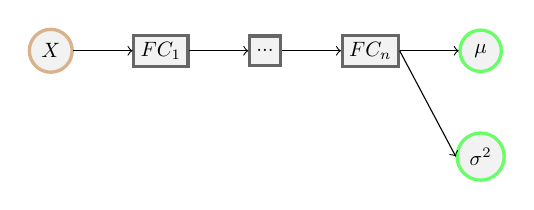
\begin{tikzpicture}[scale=0.75, transform shape,
roundnode/.style={circle, draw=brown!60, fill=black!5, very thick, minimum size=7mm},
roundnodey/.style={circle, draw=green!60, fill=black!5, very thick, minimum size=7mm},
squarednode/.style={rectangle, draw=black!60, fill=black!5, very thick, minimum size=5mm},
]
%Nodes
\node[roundnode]      (X)                             {$X$};
\node[squarednode]      (FC1)                      [right=of X]        {$FC_1$};
\node[squarednode]      (FCmiddle)             [right=of FC1]        {...};
\node[squarednode]      (FCn)                      [right=of FCmiddle]        {$FC_n$};
\node[roundnodey]      (mean)                             [right=of FCn] {$\mu$};
\node[roundnodey]      (variance)                             [below=of mean] {$\sigma^2$};

%Lines
\draw[->] (X.east) -- (FC1.west);
\draw[->] (FC1.east) -- (FCmiddle.west);
\draw[->] (FCmiddle.east) -- (FCn.west);
\draw[->] (FCn.east) -- (mean.west);
\draw[->] (FCn.east) -- (variance.west);
\end{tikzpicture}
\caption{Example of an undivided Neural Network architecture}
\label{fig:undividedarchitecture}
\end{figure}

\begin{figure}[htb]
\centering
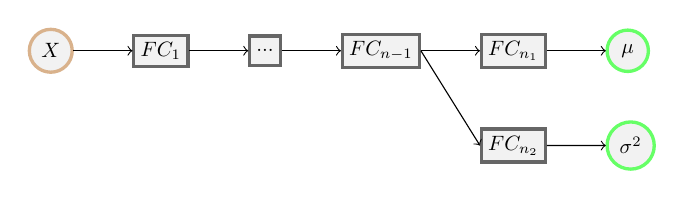
\begin{tikzpicture}[scale=0.75, transform shape,
roundnode/.style={circle, draw=brown!60, fill=black!5, very thick, minimum size=7mm},
roundnodey/.style={circle, draw=green!60, fill=black!5, very thick, minimum size=7mm},
squarednode/.style={rectangle, draw=black!60, fill=black!5, very thick, minimum size=5mm},
]
%Nodes
\node[roundnode]      (X)                             {$X$};
\node[squarednode]      (FC1)                      [right=of X]        {$FC_1$};
\node[squarednode]      (FCmiddle)             [right=of FC1]        {...};
\node[squarednode]      (FCpenaltimate)             [right=of FCmiddle]        {$FC_{n-1}$};
\node[squarednode]      (FCn1)                      [right=of FCpenaltimate]        {$FC_{n_1}$};
\node[squarednode]      (FCn2)                      [below=of FCn1]        {$FC_{n_2}$};
\node[roundnodey]      (mean)                             [right=of FCn1] {$\mu$};
\node[roundnodey]      (variance)                             [right=of FCn2] {$\sigma^2$};

%Lines
\draw[->] (X.east) -- (FC1.west);
\draw[->] (FC1.east) -- (FCmiddle.west);
\draw[->] (FCmiddle.east) -- (FCpenaltimate.west);
\draw[->] (FCpenaltimate.east) -- (FCn1.west);
\draw[->] (FCpenaltimate.east) -- (FCn2.west);
\draw[->] (FCn1.east) -- (mean.west);
\draw[->] (FCn2.east) -- (variance.west);
\end{tikzpicture}
\caption{Example of a divided Neural Network architecture}
\label{fig:dividedarchitecture}
\end{figure}

In both these figures,  FC stands for fully connected layers.
As the undivided architecture is closer to the neural network used in the proposed ranking loss surrogate model,  we used it for the sake of consistent comparison.
3 Fully connected layers of 32 neurons each were used for each neural network.
All neural networks used the same architecture. 
The training was done using the the Adam optimizer with full batch gradients.
This is because the number of data points in the evaluation cycle are very few.
Each neural network was trained for a 1000 epochs with a learning rate of 0.02.
We do not use adversarial examples as proposed in the deep ensemble paper because it was giving bad results.

\subsection{Few Shot BO: Deep Kernel Learning}
Few Shot Bayesian Optimization has to be run in 2 chronological steps
\begin{itemize}
\item Meta training using the existing meta data
\item Fine tuning during the optimization cycle.
\end{itemize}
Some of the important implementation details are
\begin{itemize}
\item Scaling is ignore because it gives very bad results.
\item We first used RBF kernel,  then we used matern kernel for this.
\end{itemize}

Scaling should be ignored because it gives very bad results.
if scaling:
%# Scale the labels according to the l and u for scale invariance.
%        #     batch_labels = (batch_labels - l) / (u - l)

%%         ## RBF kernel
 %## Another possibility of a kernel - self.covar_module =
   %     ## gpytorch.kernels.ScaleKernel(gpytorch.kernels.MaternKernel(nu=config["nu"], ard_num_dims=dims if config["a    rd"] else None))

We used early stopping mechanism for this because we wanted to avoid
\begin{itemize}
\item Huge computation costs
\item overfitting of the model during training.
\end{itemize}
We saved the best model in our implementation and if the validation loss went greater than
lowest validation loss for some number of steps,  then we stop the meta training.

\subsubsection{Implementation issues}
After completing the own implementation,  we found that the results obtained were not in par with the paper.
For this reason, the results are used only for the first stage.
The results already present in the benchmarking data of~\cite{pineda2021hpob} were used for comparing this result with our implementation.


% \section{Evaluation Strategy}



\chapter{Method}\label{chap:ProposedIdea}

\section{Proposed Idea: : Ranking Loss Surrogates}

The choice of surrogate to use in model based optimization is very crutial.
Does the surrogate have enough representational capacity?
Does it have the capability of representing uncertainty?
How is the surrogate learnt?
These are some of the questions that need to be answered before selecting a sorrogate model.
The selection of a sorrogate model has a direct impact on the performance of the model based optimization algorithm.

In the quest to improve HPO surrogates,  we propose and analyse a new type of surrogate model that is based on the concept of ranking.
There are 2 components of our proposed idea

\begin{itemize}
\item The learning mechanism of the surrogate model.
\item The surrogate model itself.
\end{itemize}

This chapter discusses in detail both these components.
In this chapter,  we first assume that a good surrogate model of sufficient representational capacity already exists.
We use a simple Deep Neural network for this purpose.
We then understand,  analyse and implement the proposed learning algorithm that uses the concept of.
We then do a simple case study of inverse mapping using the learnt model.
Finally we build a ranking model to improve the performance of any model based HPO algorithm.
We use SMBO as a reference for our study.


\subsubsection{Implemenation notes}
The implementation is done by removing top element check comments
The latest implementation is used due to its efficiency otherwise it is the same. (note)

Our implementation is given by the following algorithm
Write the algorithm of our implementation here

Implementation given by the paper~\cite{Pobrotyn2020ContextAwareLT}.
Here give the equations used by this algorithm

Main Idea:
    We need to use ranking losses instead of other methods for the purpose of HPO algorithms.


Applying this to HPOB... (With or without query)
    First learning from first search space.
    Even with this the loss curves are very smooth if we use 2 * tanh(0.01 * x)
    
    
\section{Case study}

In this case study,  we study how the learnt ranking function behaves when we use different parameters to train.
For this a toy example of sorting in reverse order is considered.


\subsection{Sorting with inverse mapping}
    
The main problem that we try to solve here is - Is it possible to train a ranking function using the Listwise maximum likelihood estimator. 
such that it learns inverse mapping of points on a number line.
Consequently we could sort the results obtained by the scorer to obtain a descending order.


Consider a list $l = \{x_1, x_2, ...x_n\}$ where $x_i \in [1, 100]$.
Let $s(x \mid \theta) \mapsto \mathbb{R}$ be our scoring function parametrised by $\theta$.
One list contains $n$ data points sampled from $[1, 100]$.
Let $\textrm{L}_{\textrm{mle}}$ represent the maximum log likelihood loss.
Using this loss function we optimize for the following equation
\begin{equation}
\underset{\theta}{\arg\min} \;\;\; \textrm{L}_{\textrm{mle}}(s(l \mid \theta),  - k * l)
\end{equation}
where $k \in \mathbb{R}$.
 
Note that second parameter of list wise loss function is scale invariance because it only uses the rank of the 
objects in the list and not the objects directly.
Hence scaling the list has no effect on the loss output.
This can be seen from the algorithm of implementation.  (refer algorithm)

%    #       Result -> Sorting possible provided the output range of the model not restricted
%    #       For now we sample train/val data from the same distribution.
  %  #   List of numbers to test with = {-1 to -100}
%    #       Result -> This is not possible because the model will map this to extreme values as it
 %   #                 is not distribution dependent.
 %   #   Check the percentage of the lists in the correct sorted order.

The validation data taken from 3 different ranges
\begin{itemize}
\item Same range as the training data $[1, 100]$
\item Completely different range as seen by the scorer during training i.e $[-100, -1]$
\item Hybrid range i.e $[-50, 50]$
\end{itemize} 

To evaluate our scorer,  we first sample the validation data from the above ranges,
We then check the percentage of the lists that are correctly sorted during our testing time.
The training batch is 100 and the results are averaged over 5 runs.

tabulate the results and Check the affect of list / batch size on the results

\begin{table} [h!]
\centering
\resizebox{\linewidth}{!} {
\begin{tabular}{ | c | c | c | c | c | c | }
\hline
\textbf{Training Epochs} & \textbf{List size} & \textbf{Learning Rate} & \textbf{In-range Acc.} & \textbf{Out-range Acc.} & \textbf{Hybrid Acc.} \\ [0.5 ex]
\hline \hline
1000 & 3 & 0.0001 & 0.99 & 0.99 & 0.99\\
%100 & 3 & 0.001 & 0.99 & 0.99 & 0.99\\
%100 & 3 & 0.01 & 0.0 & 0.0 & 0.0\\
%457 & - & Linear & 0.458 & 0.419 & 0.328\\
%457 & - & Linear Duplication & 0.460 & 0.428 & 0.327\\
%\textbf{49} & \textbf{Genetic}\footnotemark[1] & \textbf{Hyperbolic} & \textbf{$\approx$0.377} & \textbf{$\approx$0.374}  & \textbf{$\approx$0.364}\\
%40 & Pearson Correlation & Hyperbolic & 0.287 & 0.278  & 0.285 \\ 
%40 & Spearman Correlation & Hyperbolic & 0.289 & 0.294  & 0.290 \\ 
%176 & Manual & Hyperbolic & 0.362  & 0.346  & 0.331\\ [1ex]
\hline
\end{tabular}
}
\caption{Sorting Accuracies at test time}
\label {table:1}
\end{table}

\iffalse
\begin{table}[ht]
\centering
% spacing in table
% \ra{1.3}  % Commenting this could not get this function right
\begin{tabular}{@{}lr@{}}
  \toprule
  Epochs listsize & Accuracy(within range) Accuracy outside range \\ \midrule
  A    & 82.47 $\pm$ 3.21 \\
  B    & 78.47 $\pm$ 2.43 \\
  C    & 84.30 $\pm$ 2.35 \\
  D    & 86.81 $\pm$ 3.01 \\
  \bottomrule
\end{tabular}

    \caption[Table caption]{\textbf{Sorting accuracy.} Obtained after sorting the numbers based on the scorer's results\\}
    \label{tab:accuracy}
\end{table}
\fi

show the architecture of with only scorer


\subsection{Observations}
As we know that the second parameter of the loss function is not bound to any range, 
the score function itself can learn scores of arbitrary range.
Hence the model can learn score values arbitrarily large.
We must control the output domain so that the training does not lead to underflow or overflow.
This is because we use the exp function for getting the strict positive increasing function.

The restriction of output was done using $\tanh()$ so that the range of values of the scorer remains within a managable value.
One drawback we found was that the learnt model was extremely sensitive to the learning rate and the number of epochs.
% The following observations were made in the case study of sorting example
% Perhaps using other increasing positive function helps? (More reading/research required on this topic)

  
  Then we add the following components one after another

\begin{itemize}
\item Deep Set
\item Weight
\item Uncertainty
\item Different training mechanisms.
\end{itemize}

Propose using a higher list size.

\subsection{Scoring function analysis}

\subsection{Scoring function range}

\section{Optimization cycle}
Explain the training loop with an algorithm.

explain get\_batch\_HPBO implementation how it is important to have all the data sets
How it is organised into a higher order tensor
TO compute 2 things can be done
  1. View it as a 2d tensor (Done by efficient implementation)
     2. Deal with it direction (Done by us)

replace=False thing in the above function and why it is important.

\subsection{Meta training}
Give the meta training algorithm
Why all tasks are taken - 
Because we do not want bias to crop up during the training
The idea is to meta learn commonality in the search space.

\subsection{Fine tuning}\label{sec:rlfinetune}
Given the Fine tuning algorithm.
For reasons described in the~\ref{sec:restart},  we restart before fine tuning at every optimization cycle step.

\section{Ranking Surrogate Model}

\subsection{Transfer Learning}
This is the transfer HPO-B

\subsection{Using Deep Sets to build context aware models}

As discussed in the literature review,  model a whole set into a latent embedding.
For domain conditionality 
meta train in source domain (HPOB training SS)
meta test in target domain (HPOB test/val SS)

Architecture with deep sets.. Image

\subsection{Uncertainty implementation}
Mention about the requirement to use Module list.
Show the new architecture.

The search spaces that have less data need more uncertainty
The search spaces having more data need less uncertainty

\subsubsection{Independent training}
Implementation yet to be done

\subsubsection{Training with mean and restricted output}
Implementation yet to be done

\section{Requirement of restarting training}\label{sec:restart}
We find in our experiments that the deep ensemble performs much better in our HPO cycle when we train it from scratch at every acquisition step.
This is counter intuitive because an already trained model will converge to a local optima quickly.
The reason for this performance however is that the model gets biased towards the points that are observed at the beginning of the optimisation cycle.
Lets say we have 2 models 
\begin{itemize}
\item $\textrm{m}_{\textrm{restart}}$ which always restarts training at every acquisition step.
\item $\textrm{m}_{\textrm{reuse}}$ which uses the previously trained model for subsequent training of the optimization cycle.
\end{itemize}

\begin{figure}[htp]% [H] is so declass\'e!
\centering
\begin{minipage}{0.45\textwidth}
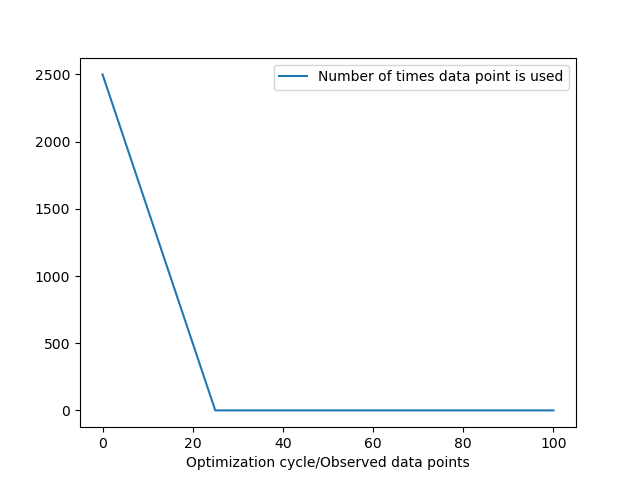
\includegraphics[width=\textwidth]{images/bias25}
\caption{Bias at 25th optimization cycle}
    \label{fig:bias25}
\end{minipage}\hfill
\begin{minipage}{0.45\textwidth}
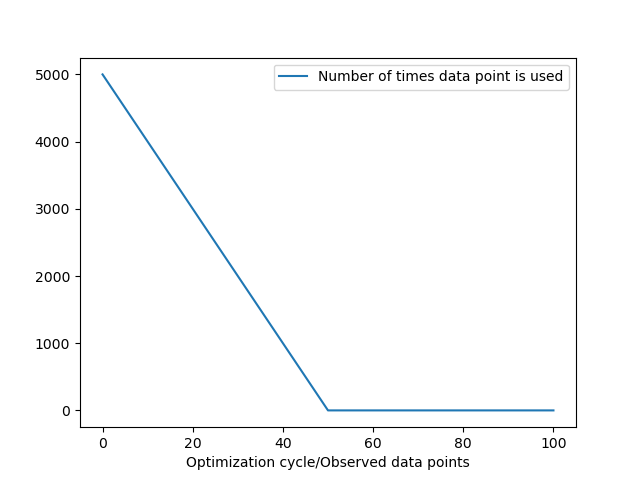
\includegraphics[width=\textwidth]{images/bias50}
\caption{Bias at 50th optimization cycle}
    \label{fig:bias50}
\end{minipage}\par
\vskip\floatsep% normal separation between figures
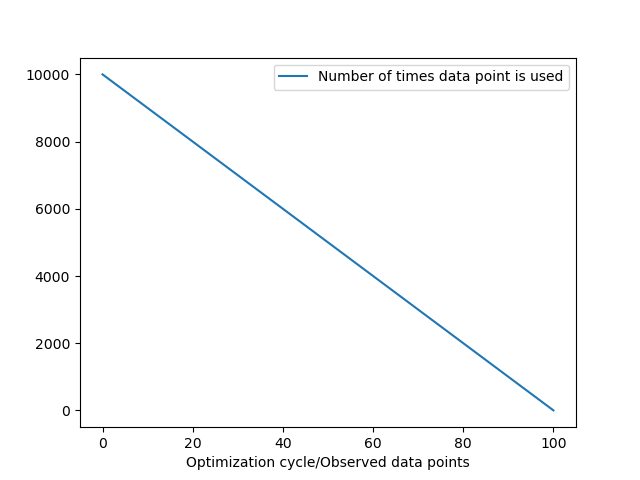
\includegraphics[width=0.45\textwidth]{images/bias100}
\caption{Bias at 100th optimization cycle}
    \label{fig:bias100}
\end{figure}


Let $\textrm{m}_{\textrm{reuse}}$ be fine tuned for 100 epochs during the optimization cycle.
Let there be just 1 data point to start with.
The figures~\ref{fig:bias25},~\ref{fig:bias50},  and ~\ref{fig:bias100} show the number of times each observed data points is used for the fine tuning at the 25th, 50th and 100th optimization cycle by $\textrm{m}_{\textrm{reuse}}$  respectively.
Generally all the data is used during fine tuning due to its scarcity at this step.
Hence, the biases are scaled with the number of epochs.
$\textrm{m}_{\textrm{restart}}$ does not face this issue as the fine tuning step restarts everytime.

The heavy bias that is present in the figures is actually not intended.
This is because all observations should be treated equally in any training/fine-tuning step.
Hence it is better to restart the model before fine tuning step at each optimization step.

The second reason is that the model may get stuck at a stubborn local minima at any fine tuning step n $1 <= n <= 100$.
Coming out of this local minima may require vastly different data points than actually seen.
This is not generally the case in our sequential optimization.

We use this restart mechanism in our ranking loss model in order to make it more robust against these issues.

\section{Weighted Loss}
General list wise loss functions are only required in the problem domains where it is essential to get the ranks of all the objects correctly.
In our case where ranking functions are used as surrogates for the black box hyper-parameter optimization,
this constraint can be relaxed significantly.
As discussed in section~\ref{sec:rlfinetune},  we always restart our ranking function model before
fine-tuning it.
Hence,  after fine-tuning we are only bothered about getting the best hyper parameter configuration from the pending configurations.
This means that it is more important for our ranking function to order the the top part of the list than the bottom part.
In this section we describe and propose the concept of weighted ranking loss functions.

The concept of biased ranking loss is discussed in the paper, "Top-Rank Enhanced Listwise Optimization for Statistical Machine Translation" by  Chen et. al~\cite{TRLWO}.
Here Chen et. al proposes a position based weighting of the ranking function such that:
\begin{equation}
w_j = \frac{k - j + 1}{\Sigma_{t=1}^k t}
\end{equation}
where $w_j$ represents weight of the object at position $j$ in the ordered list.

However, there are also some simple weightings that a person can use.  For instance inverse linear weighting given by
\begin{equation}
w_j = \frac{1}{j}
\end{equation}
and inverse logrithmic weighting given by
\begin{equation}
w_j = \frac{1}{\log (j+1)}
\end{equation}

\begin{figure}[htb]
  \centering
    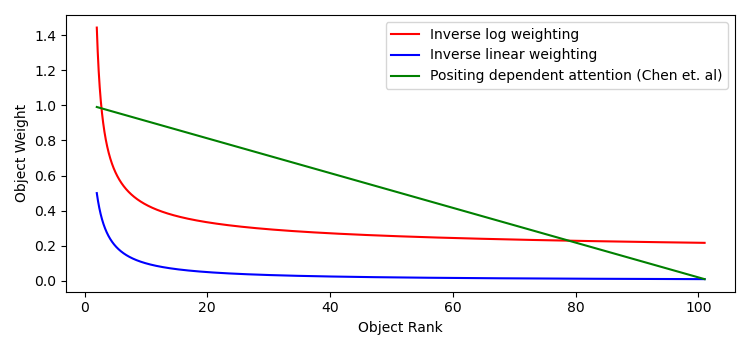
\includegraphics[scale=0.65]{images/weightingfunctions}
    \caption{Different Weighting Functions}
    \label{fig:weightingfunctions}
\end{figure}

Figure~\ref{fig:weightingfunctions} shows all 3 weighting strategies.
Of the 3 weighting strategies,  the inverse log weighting was found to be most suitable.
This is because the this weighting is by far the least sharp.
As the weighting does not decrease very rapidly,  there is a possibility of parallelizing during the optimization cycle.
For example,  at every step the top $n$ configurations can be selected,  and all of them can be tried for optimization.
The parallelism is less effective when using inverse linear weighting or weighting proposed by Chen et al.

\section{Using cosine annealing}
During the fine tuning of our models both in the baselines as well as the ranking loss model,  it was found that the fine tuning loss curve was varying a lot.


We obtained loss curves that were very bad during the training and were varying quite a bit
The reason was that the learning rate during the fine tuning was too high
Hence we used cosine annealing for this to get the a better local minima.

Show before and after curves.


The results of this are discussed in the results section.


\section{Advantages and Limitations}

Compare this loss function and method with other base lines..
Advantages of the proposed Idea:
    The amount of data instances for training is exponential in number. Which is very good for a deep learning model
    For example if we have 100 observation set and we use a list size of 15 to train our model, we will have 100C15
    unique instances to train.

Observed disadvantages:
\begin{itemize}
\item In our model,  a scorer is first learnt and then using the scorer,  we rank the set of objects in question.
When optimising the scorer,  we ignore the sorting functionality necessary to complete the process of ranking.
This is because sorting is non differentiable. 
This means that the true evaluation of the ranked list is not optimized.
This needs to be improved which is done in Pi-Rank paper.
\item The learnt model is extremely sensitive to the learning rate and the number of epochs.
\item It is assumed that the target task and the training task have the same output range. 
They must be normalized in order to get the correct results if they are not in the same range.
\end{itemize}
    
\subsection{Negative transfer learning}
For some search spaces,  the validation errors of the ranking loss model did not reduce at all during its training.
In fact the validation loss became worse.
Figure~\ref{fig:NegativeLearning} shows an illustration of this for the search space id 5527.
This is a classic example of negative transfer learning~\cite{Weiss2016}.
Negative transfer learning occurs when the set of source tasks (here,  training datasets) is very different from the target tasks (here, validation datasets).

\begin{figure}[htb]
  \centering
    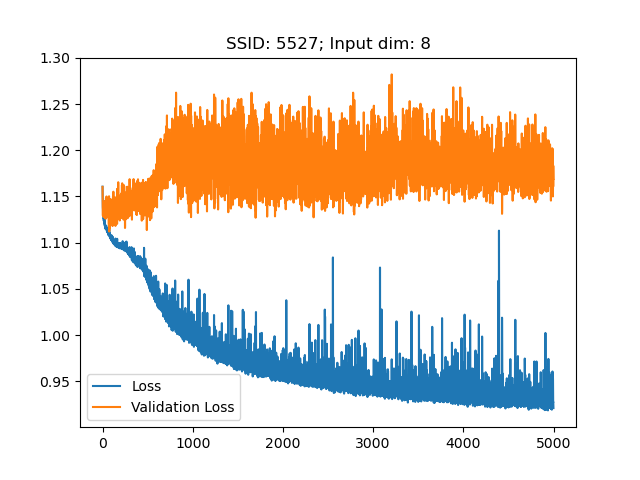
\includegraphics[scale=0.5]{images/NegativeLearning}
    \caption{Training loss curve of ranking losses}
    \label{fig:NegativeLearning}
\end{figure}

This problem should occur only in the cases where the model is context free.
In our case,  the ranking loss model with deep set is context aware and results like these were unexpected.
Hence the issues with negative transfer learning remains unsolved when using our model.
One remedy for getting around this problem is to fine tune the model with a larger number of epochs.
Nevertheless,  we cannot guarantee that the finetuning will re-learn from the small amount observed data points during the optimization cycle.

\chapter{Research Question}
The format of this is the same as that of experiments and Results.
Also known as Hypothesis

\chapter{Experiments and Results}
Evaluating a novel hyper parameter surrogate is extremely expensive.
For this,  we would have to run the HPO technique (Bayesian optimization in our case) with our surrogate on a set of different machine learning models.
This is because each ML model has a different search space.
Moreover,  the optimum within the HP search space may be different when the ML model is trained on different data sets.
Hence we further need to do multiple HP optimizations of a model each time using a different dataset.
In addition to this due to the stochastic nature of ML models as well as the surrogate models, 
we would have to run the HPO multiple times for each dataset.

\section{Benchmarking Meta-Data}

For comparing our proposed model with other HPO models we have to do the above evaluation for each of the HPO model.
As one can see,  this evaluation if done right from the training of the ML model is not feasible.
We use the HPO-B~\cite{DBLP:journals/corr/abs-2106-06257} benchmarking in this thesis.
Using this benchmark,  we do not need to train our ML models from scratch as the meta data also contains evaluations of multiple hyper parameters for different ML models and datasets.
In this section we first discuss about the organisation of the benchmarking meta data.


HPO-B is a benchmark that can be used for doing black box HPO.
It can be used for both transfer models and non transfer models.
The meta data consists of a list of (hyper-parameter) search spaces.
These are hyper parameter search spaces of single models.
The is organised in a json format with the structure illustrated in Figure~\ref{fig:metadataorganization}.

\begin{figure}[htb]
\centering
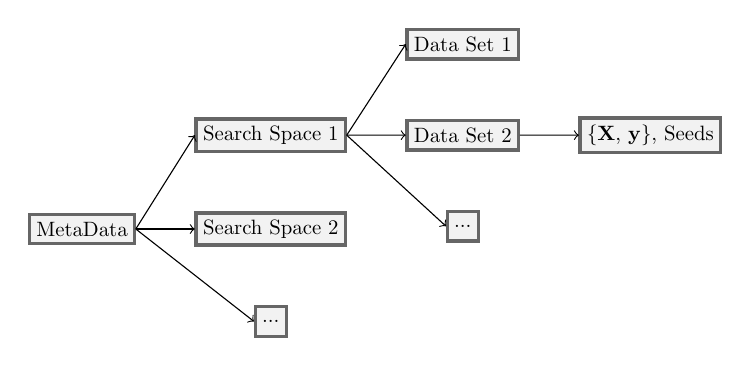
\begin{tikzpicture}[scale=0.75, transform shape,
% roundnode/.style={circle, draw=green!60, fill=green!5, very thick, minimum size=7mm},
squarednode/.style={rectangle, draw=black!60, fill=black!5, very thick, minimum size=5mm},
]
%Nodes
\node[squarednode]      (ss2)                             {Search Space 2};
\node[squarednode]      (main)                   [left=of ss2]           {MetaData};
\node[squarednode]      (ss1)                    [above=of ss2]          {Search Space 1};
\node[squarednode]      (ss_)                       [below=of ss2]        {...};
\node[squarednode]      (ds2)                       [right=of ss1]        {Data Set 2};
\node[squarednode]      (ds1)                       [above=of ds2]        {Data Set 1};
\node[squarednode]      (ds_)                       [below=of ds2]        {...};
\node[squarednode]      (Xy)                       [right=of ds2]        {\{\textbf{X},  \textbf{y}\},  \textrm{Seeds}};

%Lines
\draw[->] (main.east) -- (ss2.west);
\draw[->] (main.east) -- (ss1.west);
\draw[->] (main.east) -- (ss_.west);
\draw[->] (ss1.east) -- (ds2.west);
\draw[->] (ss1.east) -- (ds1.west);
\draw[->] (ss1.east) -- (ds_.west);
\draw[->] (ds2.east) -- (Xy.west);
\end{tikzpicture}
\caption{Structure of the meta data in the HPO-B benchmark}
\label{fig:metadataorganization}
\end{figure}
Where \textbf{X} represents the set of configurations for a evaluated for a model in a particular data set and
\textbf{y} represents the evaluation results.
The bayesian optimization used in our thesis can be started with different initial known HP configurations.
One initial configuration, called a seed in the meta data, is provided by a set of values (or indices) in $\textbf{X}$ and $\textbf{y}$.
There are a total of 5 seeds provided for a search space and dataset combination.

The meta data in HPO-B comes in 3 versions namely \textbf{HPO-B-v1},  \textbf{HPO-B-v2}, and \textbf{HPO-B-v3}.
Of this \textbf{HPO-B-v3} contains distlilled the search spaces that have the most datasets and can be split is split into train,  validation and test sets. 


The meta data set in HPOB is divided into test and train data.
Using meta dataset,  one can learn meta learn a model using the training split.
Then the model is evaluated in the testing split.
This data approach is used both in the baselines and proposed idea models.

\iffalse
\subsection{HPO-B Dataset}
To use the HPO-B code,  one must write function observe\_and\_suggest and observe\_and\_suggest\_continous to deal with discrete and continous optimisation case respectively.
Due to out of scope nature of the continous case,  in our implementation we assume that we are dealing only with the discrete case only.

The implementation of observe\_and\_suggest functions differs based on the surrogate model used by our problem.
\fi

\subsection{Benchmark evaluation}
There are 2 types of HP optimization surrogates that are studied in this thesis - transfer learning surrogates
and non-transfer learning surrogates.
This benchmark can be used for analysing both types of models.
However,  in order cross compare transfer and non-transfer techniques,  we only compare against HPO-B-v3 test split as recommended in the HPO-B paper.

Data used in the experiment
Infrastructure used
(That is the protocol)
Results should be structured like hypothesis.

experiment and results
protocol
data split…

First show the resutls of implementation of GP (M = 5 and M =10 )
Benchmark this...

Next with DKT (Benchmark this)

Next show the best results obtained by architecture.

\section{Evaluation}
\subsection{Testing}
explain how a ranking graph works ar implemented
Explain the regret rank@ some location.

\subsection{Ablation}

Result tabulation of case study: sorting:
1.  Within range
2.   Outside range 
mean of 3 times should be written.

show the results of raw without deep set.

Next show different strategies used for building the ranking loss model one step at a time.
First with only scorer.
then with deep set.
Then with raw deep set
fine tuning and deep set
adding uncertainty

Checking the early stop and hypothesing why is was wrong.

box plot variation of each of the scorers... for 1 or more data sets?

show results of independent training and training with output restriction

what about training independently,   this requires normalization. 
as explained by sebastian.

\chapter{Conclusion}


\section{Further work}
Further study required with other baselines that deal with ranking loss.

In our methods we used the ensemble of DNNs which output a list of results.
We use this results to calculate the mean and the variance of our  prediction.
However,  the deep ensemble paper proposes a method to directly calculate the mean
and variance.
However,  the integration of this idea with ranking losses is non-trivial.
Hence the usage of this type of loss with the ranking loss function can be taken up in further research in order to check whether their is improvement in the results or not.

Working with continuous HP spaces.
How about dividing the space into areas and use 1 HP configuration as a representative
of the space (in the euclidean sense)
Then select the best region and subdivide the space and continue the process.
There are limitation,  cannot really guarantee the optima will be found like the gradient methods.
Hence this method is suboptimal to the gradient based HP methods for continuous search spaces.

\iffalse
Paper: https://arxiv.org/pdf/2012.06731.pdf
       (Impt Ref) https://arxiv.org/pdf/1903.08850.pdf

Key Idea:
    Use permutation matrices to represent sorting. Learn the matrix with the loss function.
    [0 1 0] [x]    [y]
    |1 0 0| |y|  = |x|
    [0 0 1] [z]    [z]
    Permutation Matrices are not smooth in the input space Hence relaxation is necessary for differentiability
    Relaxation is done by using a double schocastic matrices i.e all row and column matrices sum to 1.

    Unimodal
    Double schochastic

The idea of Permutation Matrices is taken from Neural sort - Neural sort (Impt ref)

PLACKETT-LUCE DISTRIBUTIONS -> Very important to explain the rationale about using score as a probability
    measure for our scoring function (Check section 2.1 of paper 2 (Neural Sort))
\fi 
 
\section{Conclusion}

\bibliographystyle{plain}
\bibliography{references}
\pagenumbering{roman}

\appendix
% \chapter*{Appendices}
\chapter{More information}
This thesis was completed in the representation learning lab of Albert-Ludwig-Universität Freiburg.  (Figure~\ref{fig:UniLogo})

\begin{figure}[htb]
  \centering
    \includegraphics[scale=0.35]{images/logo}
    \caption{Logo: Albert-Ludwig-Universität Freiburg}
    \label{fig:UniLogo}
\end{figure}

\end{document}

